\begin{figure*}
	\centering
    \resizebox{1.5\columnwidth}{!}{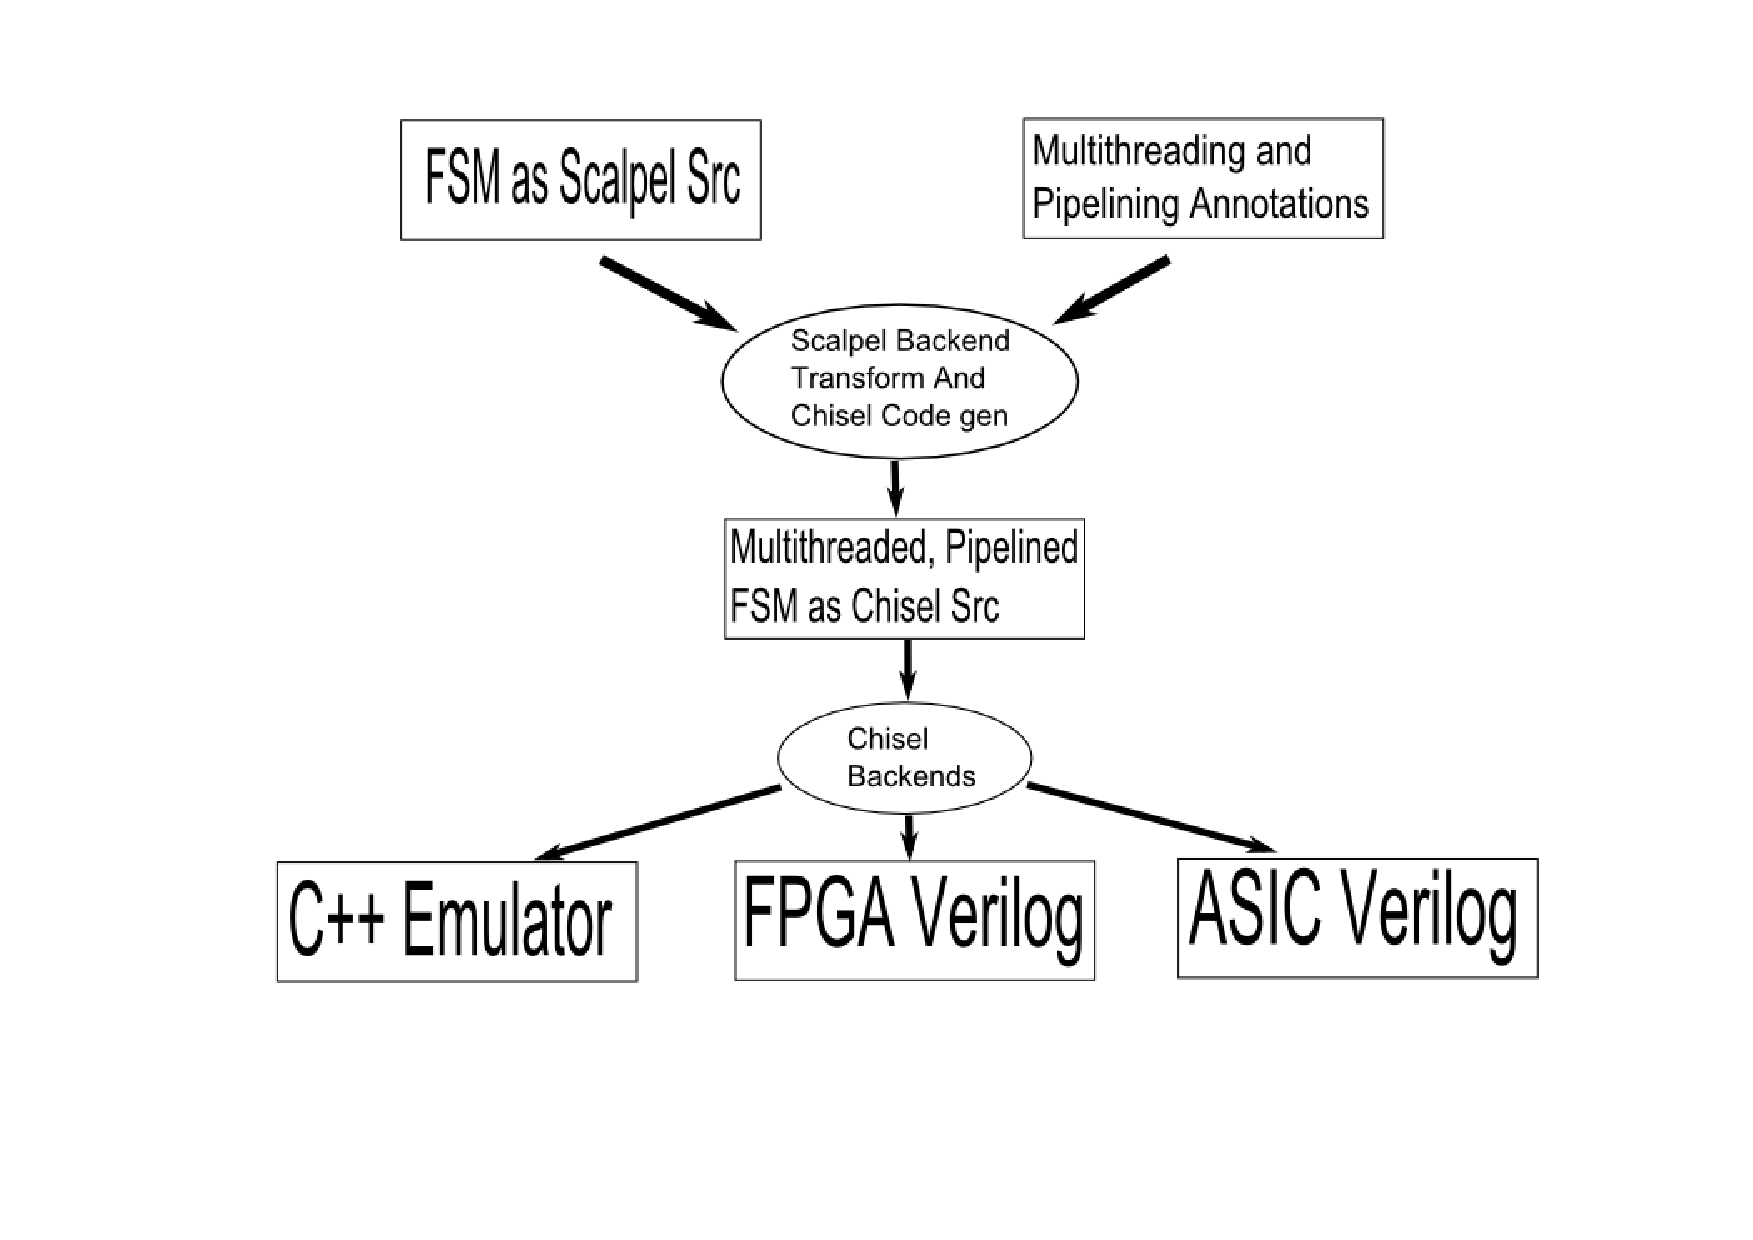
\includegraphics{figures/workflow}}
    \caption{The overall tool flow}
	\label{fig:workflow}
\end{figure*}
ßß
\section{Proposed Solution}
HLS produces designs with unacceptable performance/power/area tradeoffs because the synthesis tool has to solve the computationally difficult problem of formulating a datapath that executes the dataflow graph and fits within the given performance/power/area constraints. HLS tools do synthesize well optimized designs for specific patterns that occur in the high-level specification, so hardware designers working with HLS find themselves tuning high-level code to make specific synthesis tools produce exactly the datapath they want. 

This is clearly a case of automation trying to do too much. The HLS tools have a hard time formulating optimized datapaths, so the designers have to essentially tell the HLS tools what datapath they should use in a roundabout way by tuning the high-level specification. Clearly, designers would be more productive if they can specify the datapath directly. 

It seems like this conclusion tells us that designers should just do logic design using RTL in the traditional manner. However, much of traditional RTL specification deals with issues outside of simple datapath design. Logic designers spend much of their time specifying additional logic required to make the datapath fit performance/power/area constraints. Some common optimization techniques include time-multiplexing functional units, pipelining, multi-threading, out-of-order execution, etc. These commonly used datapath optimization techniques can be captured as algorithms and applied automatically.

This paper proposes a system in which the designer specifies in RTL a minimally complex finite state machine (FSM) that is functionally correct , but has no optimizations applied to it. The designer then annotates the minimal circuit with desired optimizations in the RTL source file and uses a software tool to automatically apply the optimizations to the minimal FSM. It is useful to have the annotations that specifiy optimizations to be used be placed directly in the RTL src file because it allows the user to refer to variables present in the RTL when specifying ooptimizations. The tool described in this paper is capable of creating multi-thread in-order designs of any number of threads and any number of pipeline stages that is functionally equivalent to n-copies of the original minimal FSM, where n is the number of threads.

The RTL specification language used in this paper is a reduced version of Chisel\cite{Bachrach:2012}, a HDL developed by UC Berkeley. A reduced version of Chisel is used for this paper to help constrain the scope of the project and to produce initial results. This reduced version of Chisel will be refered to as Scalpel for the rest of this paper. In the future, the system will be extended to work with Chisel.

The automatic optimization tool described in this paper extends a previous class project that implemented a system that automatically generates in order pipelined designs from a minimal FSM specified in Chisel. There are many shared features and components between this tool and the old tool. The remainder of the paper will focus on the automatic multi-threading parts of the tool.

Figure \ref{fig:workflow} shows the flow of the entire system. The designer first creats a ISA simulator like minimal FSM that does not have optimizations implemented. Then the designer specifies
The automatic optimization tools discussed above work in the following manner. First, some initial processing transforms the RTL specification of the base datapath into a node graph data structure, where each node represents a digital circuit component(wire, combinational logic block, or state element) and each node contains input and consumer pointers to other nodes representing the topology of the circuit. Second, the tools implement the specified optimizations by modifying this node graph - creating new nodes, changing input/consumer pointers, copying existing nodes, etc. Third, the tool outputs the modified circuit in some specified representation
 

